%   HEADERS     {
\documentclass{article}
%\documentclass[main.tex]{subfiles}
\usepackage{graphicx}
\graphicspath{ {./Images} }
\usepackage{pdfpages}
\usepackage{amsmath,amsthm,amsfonts,amssymb,amscd}
\usepackage{lastpage}
\usepackage{enumerate}
\usepackage{fancyhdr}
\usepackage{mathrsfs}
\usepackage{xcolor}
\usepackage{graphicx}
\usepackage{listings}
\usepackage{caption}
\usepackage{sectsty}
\usepackage[subpreambles=true]{standalone}
\usepackage{import}
\newcommand\tstrut{\rule{0pt}{2.4ex}}
\newcommand\bstrut{\rule[-1.0ex]{0pt}{0pt}}
\usepackage[margin=1in,includefoot]{geometry}
\pagenumbering{gobble}
%}
%   REPORT      {
\begin{document}
%   PURPOSE     {
\section*{Purpose}
The main objective for the lab activity ,``\textbf{ Measuring Permittivity of Free Space} '' is to predict the capacitance of an isolated capacitor to an exact measure and to compare calculated \& theoretical permittivity of free space. Using a few items such as a spherical conductor, a ground, a capacitance meter , and a ruler to enable comparisons from calculated and measured permittivity of free space.

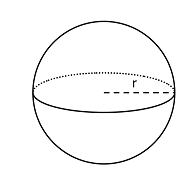
\includegraphics[scale=.7]{Images/sphere.png}
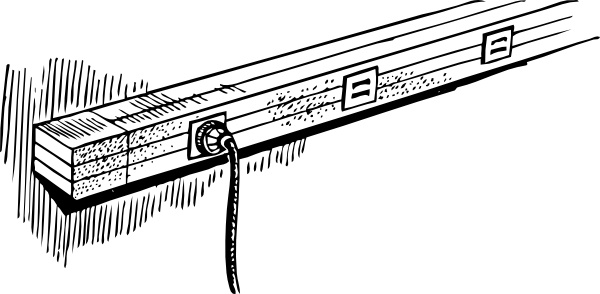
\includegraphics[scale=.2]{Images/powerstrip.jpg}
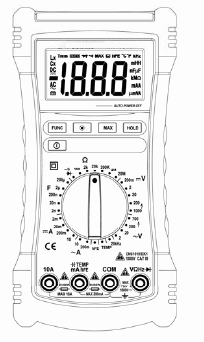
\includegraphics[scale=.35]{Images/meter.png}
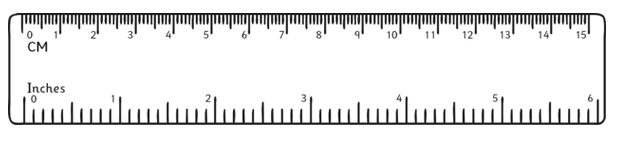
\includegraphics[scale=.3]{Images/ruler.png}
\vspace{1cm}

There are two general operations for this lab which are to : obtain a isolated conductor, place a positive charge $Q+$ on the conductor, compute the electric field using Gauss' law to gather how electricity flows within a surface {(which is spherical)} $ \therefore \ E_{\text{\scriptsize{sphere}}} = \frac{Q+}{4\pi \epsilon_{0} r^{2} } $, obtain the potential difference $\Delta V$ to get a capacitance $C = \frac{Q}{\Delta V} $ using that information.  The other operation for this lab is to exhibit the theoretical result of measuring permittivity of free space  and compared permittivity of free space by developing a linear relationship linking the capacitance between two parallel plates and the separation between plates. Using spacers, measurements, and the capacitance equation $C = \frac{\epsilon_{0}A}{d}$ to analyze and compare the permittivity of free space(s) from the two parallel plates.
%}
%   THEORY      {
%\newpage{}
\section*{Theory}
\subsection*{Capacitance of a Spherical Capacitor}
There are several calculations and expressions that need to be addressed before continuing with procedures. Permittivity of Free Space, Gauss' Law, Potential Difference, and Capacitance all have a mathematical equation and few concepts that need to be understood. Permittivity of Free Space $\epsilon_{0}$ can be represented as how much electric flux (or flow of electricity within a surface) an object can allow. Gauss' Law express as $\oint^{b}_{a} E \cdot dA$ and for a sphere the radius has the same magnitude across the surface.
\vfill

$$\phi \textit{\scriptsize{electric flux}} = EA = E4\pi r^{2} = \frac{Q}{\epsilon_{0}} \rightarrow EA = \frac{Q}{4\pi \epsilon_{0} r}$$
Once the electric field of conducting sphere is gathered. Determining the potential difference (voltage) is needed to express the relationship between potential energy, the charge, and the capacitance. Potential difference is found by integrating the electric field along the sphere. $\oint^{a}_{b} \vec{E} \cdot d\vec{l}$. {\small\selectfont \textcolor{gray}{\textit{{Notice that $\frac{Q}{4\pi \epsilon_{0}}$ is a constant within the integral leaving the radius to be integrated.}}}} 
\vfill

$$ \Delta V = \frac{Q}{4\pi\epsilon_{0}} \oint^{b}_{a} \frac{1}{r^{2}} dr \quad \rightarrow \quad  \frac{Q}{4\pi \epsilon_{0}} \left[ \frac{1}{a} - \frac{1}{b} \right] $$
\vfill

Capacitance of a conductor is the ratio of charge on the potential difference. Take the limits from $a$ to $b$ where $a$ goes to our radius and the $b$ goes to infinity. Doing this calculation shows that the charge is spread out over the surface of the sphere. $$ C = \frac{Q}{\Delta V} \rightarrow \frac{4\pi \epsilon_{0}}{\left[ \frac{1}{a} - \frac{1}{b} \right]} \rightarrow \lim_{(a,b)\to(r,\infty)} \frac{4\pi \epsilon_{0}}{\left[ \frac{1}{a} - \frac{1}{b} \right]}$$ 
\vfill

\begin{center}
    Resulting that the capacitance of an isolated conducting sphere is symbolically expressed as 
    \fbox{${C = 4 \pi \epsilon_{0} R}$}
\end{center}

With this equation, use the radius to compute the calculation and compare with the actual capacitance measurement from the  capacitance meter. 
\subsection*{Parallel Plate Capacitance}

Continuing the measuring of Permittivity of Free Space, parallel plate capacitors have been introduced to the experiment. Given the equation: $ C = \frac{\epsilon_{0} A} {d} $ where $C$ is the capacitance, $A$ is the area of one of the plates, and $d$ is the separation between the plates. The inverse of separation is used to develop a linear graph such that the slope  is expressed as $\epsilon_{0} = \frac{m}{A} \text{ where rearranged is : } m = A\epsilon_{0}$
$$ y = mx+b \rightarrow \qquad  \frac{1}{d}= (A\epsilon_{0}) \ C + 0 $$
Understanding that the variables that are controlled are the x-axis thus x = (1/d) the inverted separation distance and the y is dependent leading it to be the capacitance.
yielding the general linear form of the equation:
\begin{center}
    \fbox{$C = \epsilon_{0} \frac{1}{d}$}
\end{center}
%}
%   PROCEDURE   {
\section*{Procedure}
Before starting the lab procedures there are a few measurements that need to be obtained before doing the experiment. In the lab room there should be an isolated metal spherical conductor within the room. Obtain the radius of the spherical conductor by measuring across the surface  then $\div \ 2$. After getting the radius a positive charge needs to flow within the surface, therefore, place a charge by identifying the isolated conducting sphere is grounded, connecting a insulated wire from a power strip to the a capacitance meter (this is the positive wire), and then placing the ground wire onto the conducting sphere. 
\begin{center}
    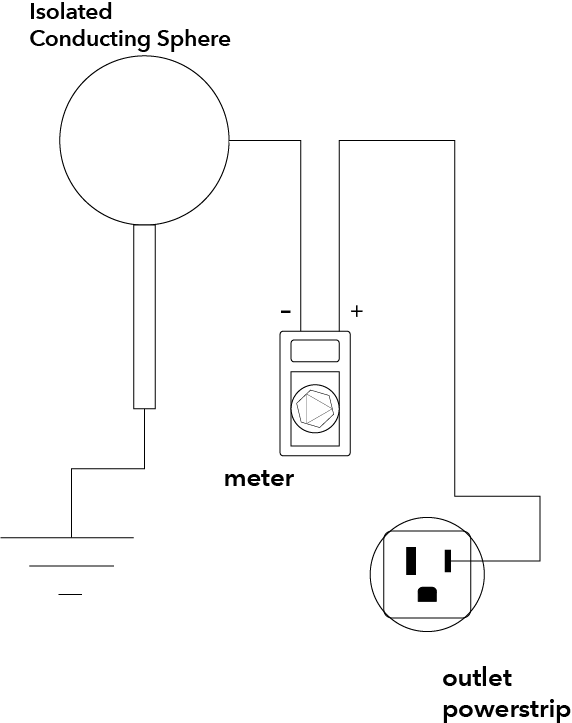
\includegraphics[scale=.25]{Images/isolatedsphere.png}
\end{center}
\break
The setup of the station is illustrated above. Furthermore, zero out the capacitance meter before reading the measurements. Once this is done compare the results from the calculated values and the measure values.If the procedures are done correctly the measurements should be similar to the capacitance calculated. In the case of this experiment: the radius of the sphere was $12.7 cm$ converted to meters to be $.127m$ where we used the equation $C = 4\pi\epsilon_{0}R \ = \ 4\pi\epsilon_{0}(.127m) \approx 1.4 \times 10^{-11} \equiv \ \fbox{14 pF}$ in result from this experiment the two measurements of capacitance is the same. Proving that the equation is generally valid in theoretical prediction and confirmation.
\vspace{1cm}

In the next set of procedures, two (17.52 cm x 17.52 cm) conductive plates are going to be used to find the permittivity of free space by using the capacitance, and a few spacers. Setup two planes with the spacers (2.11 mm thick) on the edges of the corners of the conductive planes. Connect the a positive wire to the meter and to a plane and then connect the opposite plane with a negative wire reverting back to the meter in the negative slot on the meter. Capture the capacitance, by first zeroing the meter then setting the meter to 20mA to see what the Farads are. Do this 6 times with increasing the amount of spacers each iteration by one.  

{\textit{\footnotesize\selectfont{note: do not re-zero out the meter each iteration, do it only once.}}}
\begin{center}
    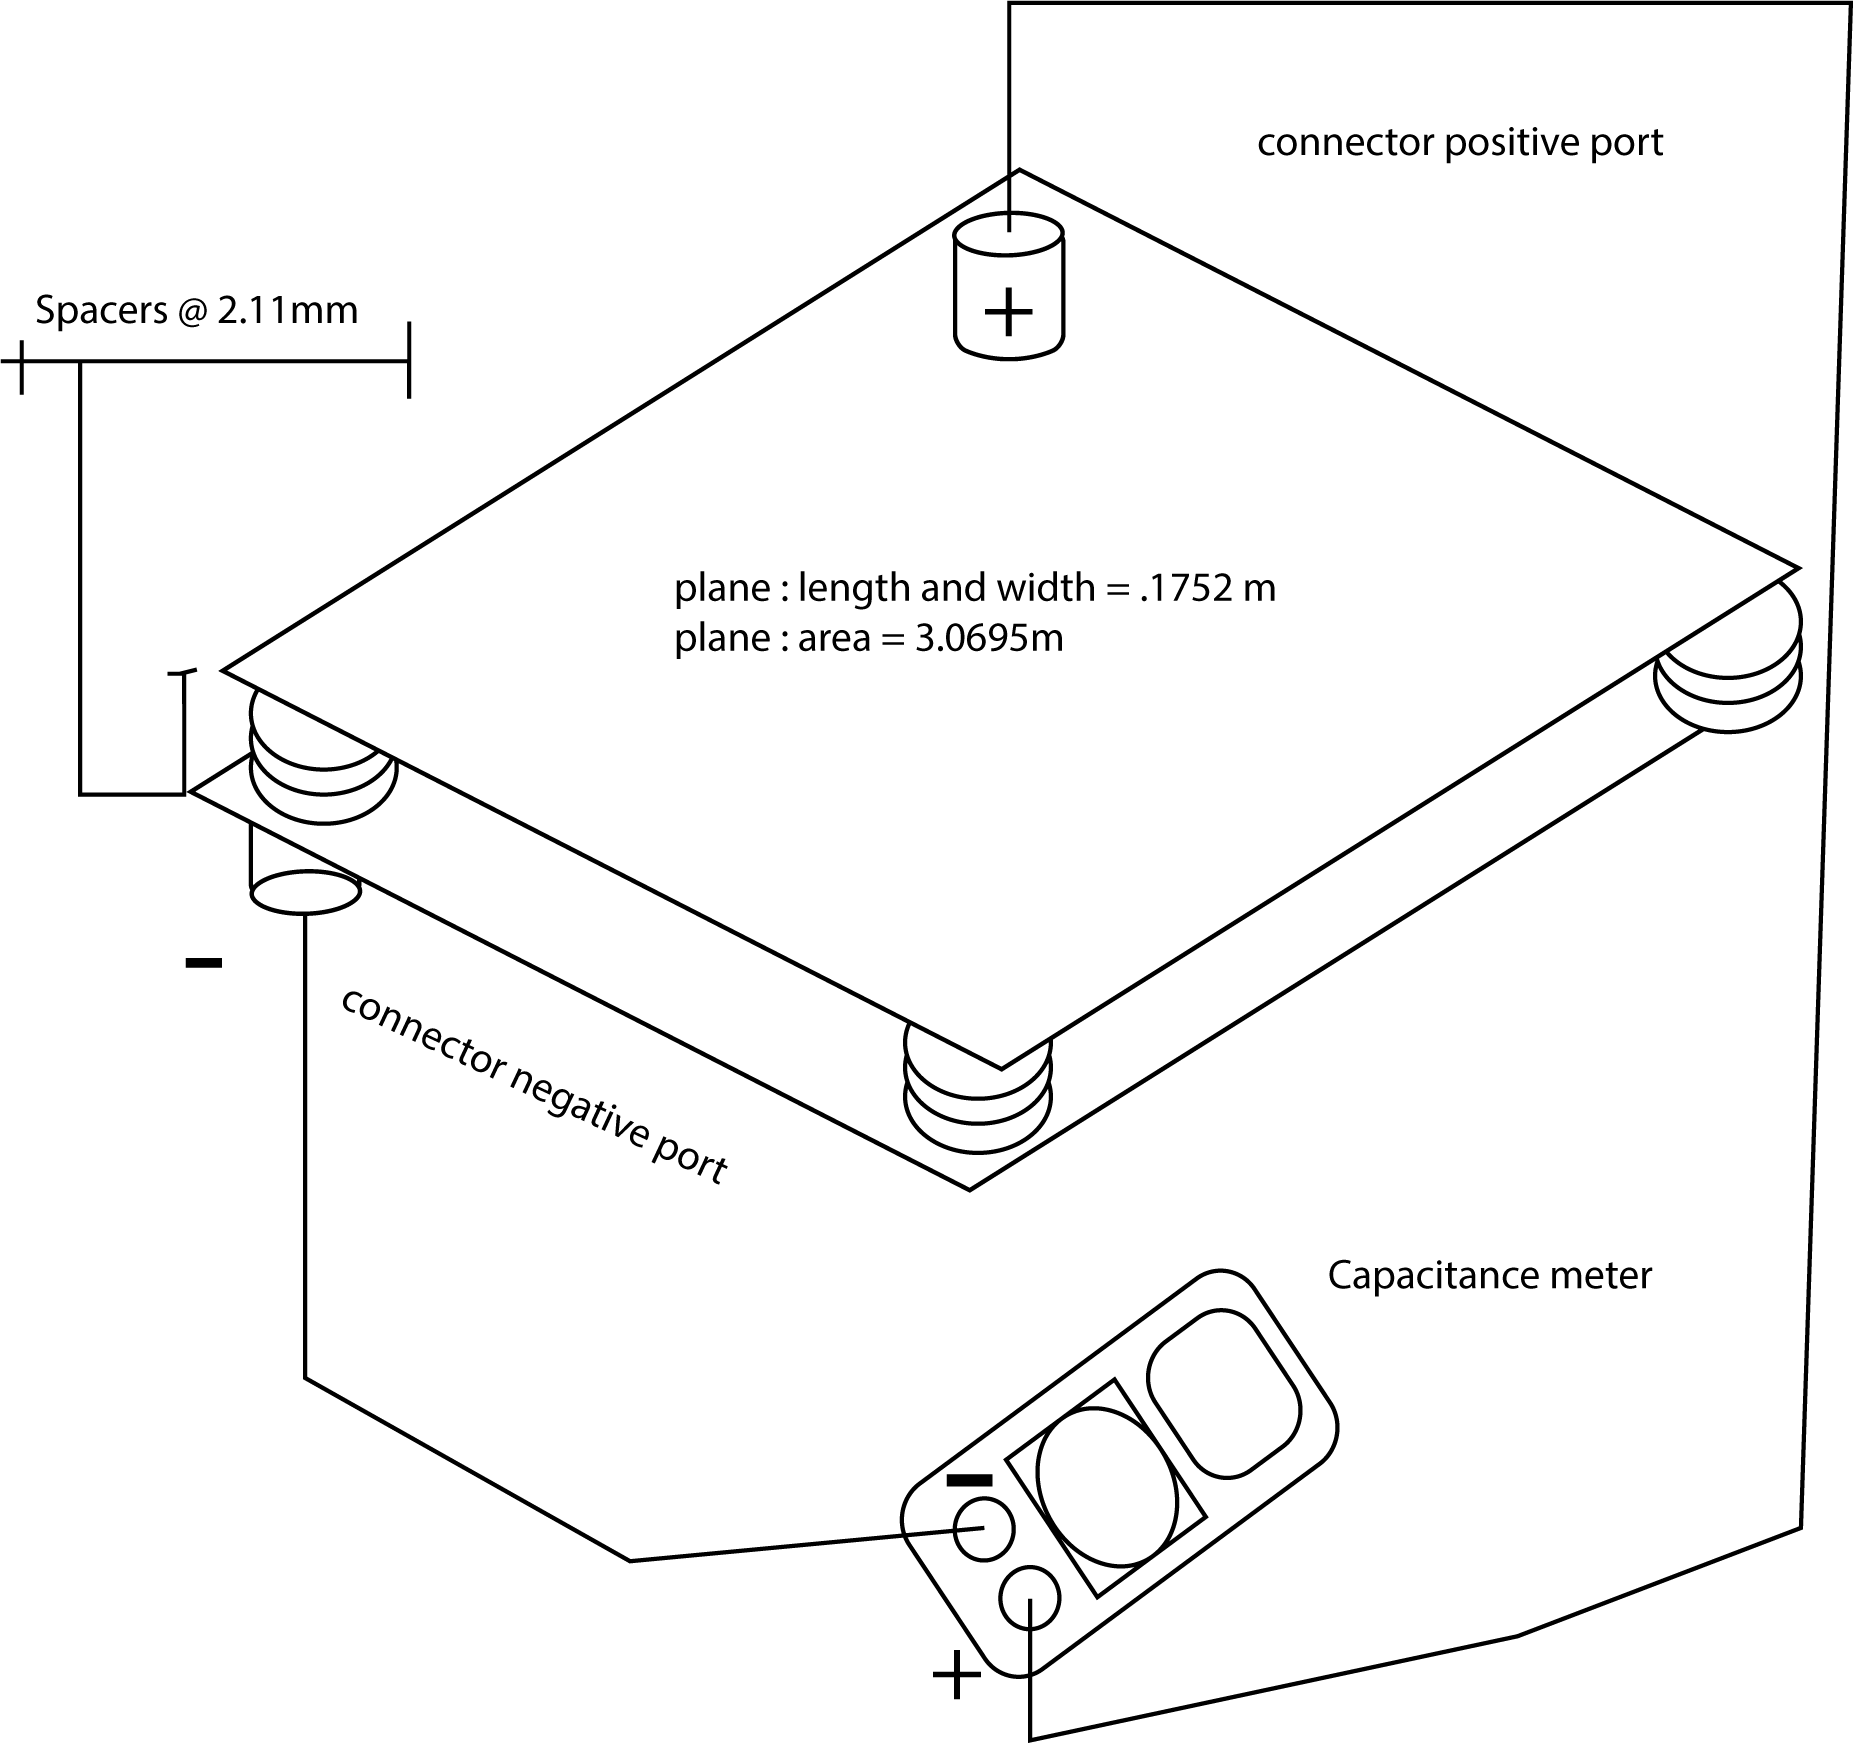
\includegraphics[scale=.4]{Images/parallel.png}
\end{center}
Record the different amounts of Capacitance and collect the data to continue the experiment.

%}
%   DATA        {
\section*{Data}
\subsection*{The Measurements: Parallel Planes}

Identify the Area of the plane(s):
$$A_{plane} = 1.752^{2}m$$
Where slope is equal to the theoretical permittivity of free space $\text{slope } = A \cdot \epsilon_{0} = 3.069 \times 8.85\times10^{-12} = 1.79 \times 10^{-12}$
%2.7165\times10^{-11}$
$$\epsilon_{\text{theoretical}} = 1.79 \times 10^{-12}$$
\vspace{.5cm}
\vfill
\begin{table}
\begin{center}
    \caption*{\underline{Measurements of Parallel Planes}}
    \begin{tabular}{ c| c| c| c |c}
     Spacers & Separation $d(cm)$ & Separation $d(m)$ & $\frac{1}{d}$ $(m^{-1})$ & Capacitance $(F)$\\
     \hline
      1 & $0.211$   &   $2.11\times10^{-3}$   & $473.93$    &  $156\times10^{-12}$  \\ 
      2 & $0.422$   &   $4.22\times10^{-3}$   & $236.96$    &  $82\times10^{-12}$   \\
      3 & $0.633$   &   $6.33\times10^{-3}$   & $157.97$    &  $63\times10^{-12}$   \\
      4 & $0.844$   &   $8.44\times10^{-3}$   & $118.48$    &  $58\times10^{-12}$   \\
      5 & $1.055$   &   $10.55\times10^{-3}$  & $95.23$     &  $49\times10^{-12}$   \\
      6 & $1.266$   &   $12.66\times10^{-3}$  & $79.36$     &  $44\times10^{-12}$   \\
      \hline
    \end{tabular}
\end{center}
\end{table}

\vfill
\begin{center}
    
    \subsection*{Capacitance vs Inverse Separation}
    \textit{Graphical Correlations}
    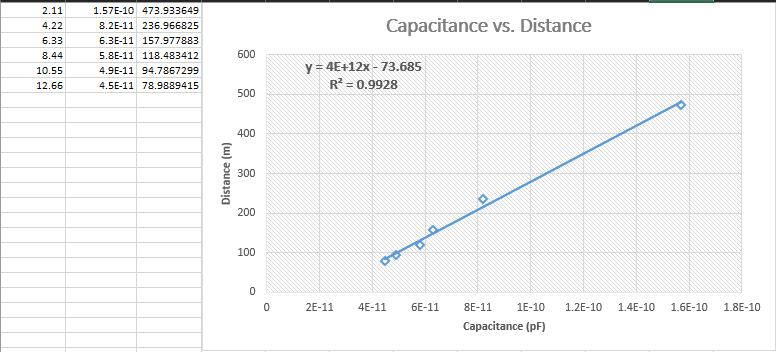
\includegraphics[scale=.7]{Images/graph.png}
    $$m  = 4 \times 10^{12}$$
\end{center}
\vfill
Using the Area ($A$) to compute $\epsilon_{0}$ from the slope : 
$$\text{slope} = \frac{A}{\epsilon_{0}}$$ 
solve for $\epsilon_{0}$ :
$$\frac{4\times10^{12}}{3.0695m^{2}} = 1.3031 \times 10^{12} \frac{C^{2}}{Nm^{2}} $$
\vfill
%}
%   ANALYSIS    {
\section*{Analysis}
Once calculations are done, identifying the percentile of error to see if the calculation are suffice and accurate enough. The experiment needs a deviation of at most 15\%. Using the formula:
$$ \text{error percentile} = \frac{ ( \epsilon_{\text{measured}}-  \epsilon_{\text{calculated}} )}{\epsilon_{\text{calculated}}} \times 100\% $$

$$ \frac { 1.31\times10^{12} - 1.79\times10^{-12}}{1.79\times10^{-12}} \times 100 \% \text{ error } = 7.32\%.$$

This is below our cap on error deviation. $7.32\% \leq 15.0\%  \quad \fbox{\checkmark}$\\

Nonetheless, identifying the different factors that hinder the data is necessary to full understand what can happen when this experiment is replicated. In general there could be factors that intervene with the experiment such as electrical interference (magnetic cards, phones, or radiating fields/frequencies), spacer positioning on the parallel plans (possibly disrupt the readability of the current it receives) , using infinite planes rather than a finite plane (clear calculations) , or insufficient groundings (the general conducting sphere not grounded correctly or one of the insulated wires are misplaced). These are some factors that could complicate your calculations. 
%}
%   CONCLUSION  {
\section*{Conclusion}
 Looking back this experiment involves different ways to measure Permittivity of Free Space, whether its through some calculations or a simple setup. Identifying the different aspects Permittivity of Free Space relates to which from electric charges, surfaces, materials, electric fields, electric currents and flows. The first part of the lab goes through calculating the capacitance of an isolated conductive sphere. Setting a charge through the conductor, computing the electric field through Gauss' Law, computing the potential difference and then evaluating the capacitance.  The second part of the lab goes over how to measure capacitance of a set of parallel planes. While doing this, the lab identifies a relationship that correlates with the permittivity of free space. This correlation is the measured permittivity of free space that is created through the data. Afterwards the correlation is compared with the theoretical. There was a slight error in the experiment but nothing to extreme. There could be multiple variables that could hinder the data, which would be unlikely to reduce in the current setting we are in. Regardless, this the experiment of Permittivity of Free Space where the exploration of electric flow is evaluated and observed.
 %}
\end{document}
%               }




%   -----------------------------------
%   created by logan malachi campbell
%   designed for reports
%   -----------------------------------
%   --------------------------
%   loganmcampbell@hotmail.com
%   www.loganmcampbell.com/
%   --------------------------